%%%%%%%%%%%%%%%%%%%%%%%%%%%%%%%%%%%%%%%%%%%%%%%%%%%%%%%%%%%%%%%%%%%%%%
%%                     Catalysis
%%%%%%%%%%%%%%%%%%%%%%%%%%%%%%%%%%%%%%%%%%%%%%%%%%%%%%%%%%%%%%%%%%%%%%
%\color{blue}
\subsection{Glyph: \glyph{Catalysis}}\label{sec:catalysis}

A catalysis is a particular case of stimulation, where the effector affects
positively the flux of a process represented by the target process. The positive effect on the process is due to the lowering of the activation energy of a reaction. The target extremity of a \glyph{catalysis} carries an empty circle.

\begin{figure}[H]
  \centering
  
\includegraphics[scale = 0.5]{images/catalysis}
  \caption{The \PD glyph for \glyph{catalysis}.}
  \label{fig:catalysis}
\end{figure}

The example in \fig{catalysis-MAPK} illustrates the use of \glyph{catalysis} arc to represent the effect of MAPKK on the phophorylation of MAPK.

\begin{figure}[H]
  \centering
  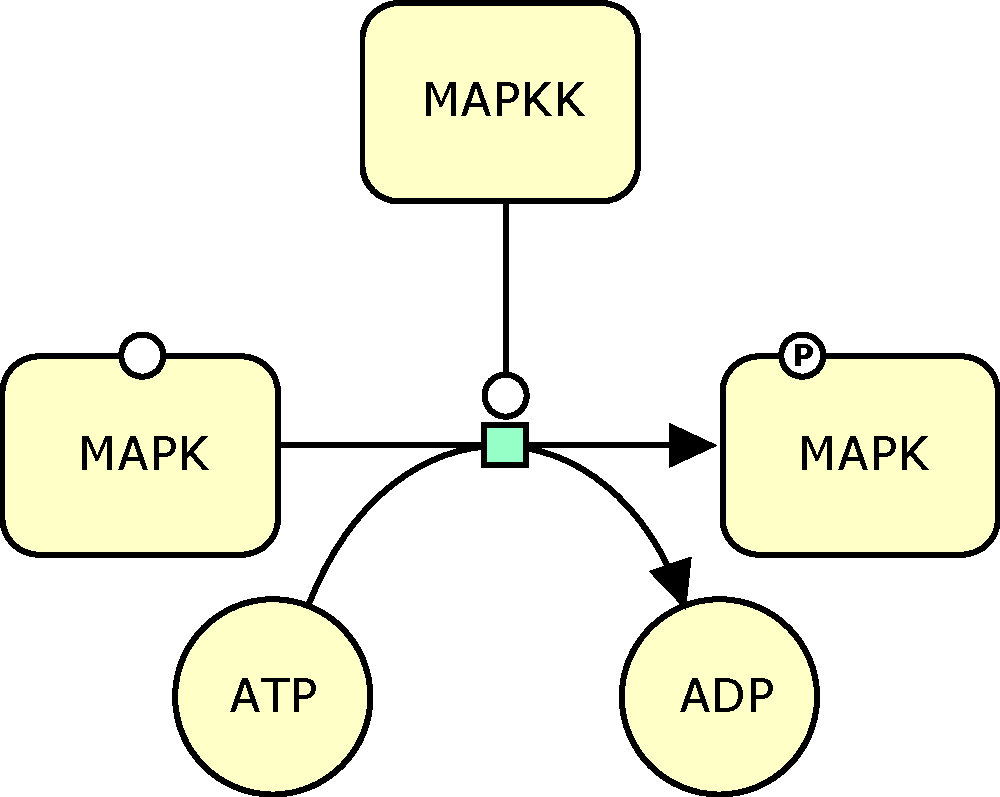
\includegraphics[scale = 0.5]{images/catalysis-MAPK}
  \caption{MAPKK catalyses the phosphorylation of MAPK.}
  \label{fig:catalysis-MAPK}
\end{figure}
